%\addcontentsline{toc}{chapter}{Development Process}
\chapter{Design}

Once an idea of which technologies to use in the software became prevalent, a design and structure of the application had to be created, based upon the requirements and user stories outlined in Appendix A, section~\ref{user_stories}. This involves a 'big picture' overview of each component of the application, where it is judged as to how to split the components. Later on in the design stages, planning, including through the use of entity-relationship modelling, and class diagrams for object-oriented components, was carried out on each specific component of the software.

This chapter will discuss the design choices made, and link them to the software's requirements. It will include any diagrams that were completed as part of this.
\newpage
\section{Overview}

\subsection{Architecture}
\begin{figure}[!ht]
	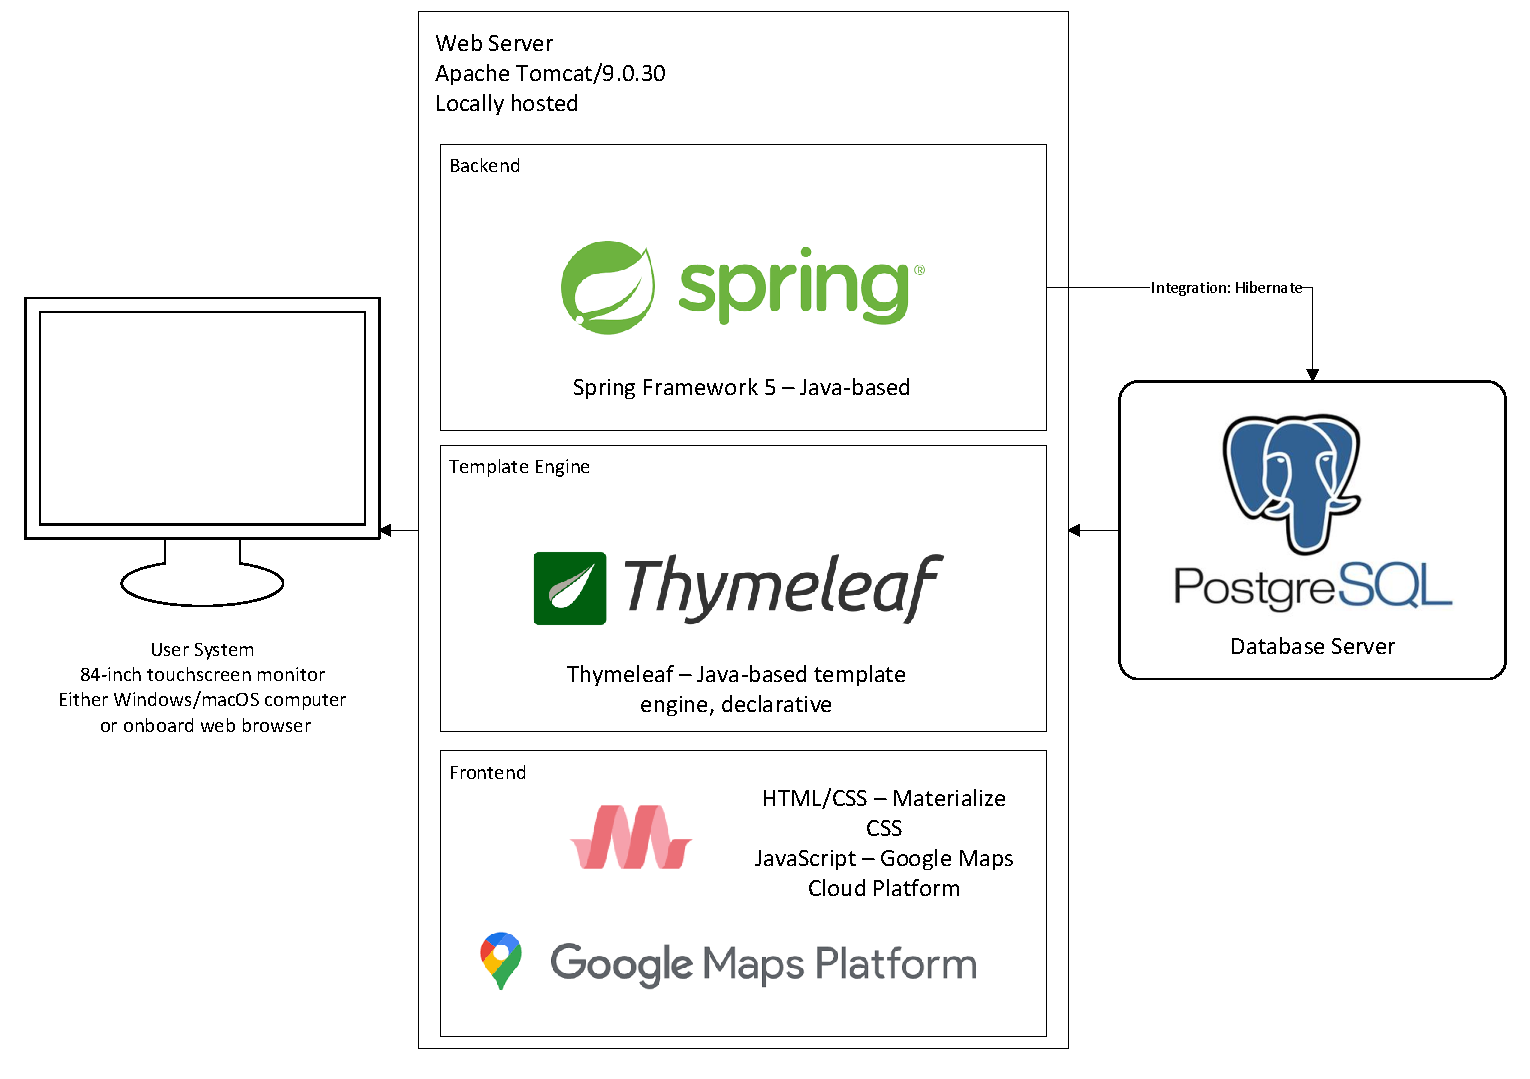
\includegraphics[scale=0.5]{diagrams/architecture_diagram}
	\caption{Architecture diagram for the Dyfi Wildlife Centre Web App}
\end{figure}	

Developing an architecture diagram ensured that there was a definition to the technology stack that the application is going to use. It also allowed for some prior thought to how different components interact with eachother.

For example, the database management system being used is PostgreSQL. Unlike systems such as SQLite, which is generally provided as a standalone file, PostgreSQL requires its own server instance. Therefore, research had to take place as to how the backend, running on Spring, would interface with the SQL Server. As evidenced in Figure 2.1, this was through Hibernate, an implementation of the standard Java persistence API for Spring's enterprise-level dialect. This was marked as something to research when planning the design for the model and controller layers of the backend.

The architecture diagram also identifies the relationships between each component hosted on the web server, in a downwards fashion. The Spring Framework interfaces with Thymeleaf, through Spring passing parameters to Thymeleaf templates, for them to be rendered. The frontend and User Experience components of the application are clearly defined - with Materialize being used for the CSS layout, and the Google Maps Cloud Platform's JavaScript API being used for displaying the map and its markers. On the left-hand side, the user's system is explicitly mentioned, as User Experience is an important consideration in this project. The user will also be interacting directly with the system and its various components that are locally hosted on the web server.

\section{Database}

Parts of the database model were able to be generated automatically using the Spring Data JPA, however it was decided that a pre-built implementation of the database model would be easier to implement, as this would ensure adherence to an entity-relationship diagram, as well as any constraints that had been identified.

The initial iteration of the database, to fulfil the first two tasks that had been defined, was to have a single relation containing details about a Point of Interest. It was decided to initially plan the database in un-normalised form. This was to ensure that the Java object that was to be created in the back-end was readable and easy to maintain, rather than having to create multiple Java objects that represent a large number of relations in the database.

The database was to be iterated upon. To allow for authentication, separate tables for users and roles were to be created. While the consideration with regards to authentication was that every user should be automatically granted admin permissions, the role database allows for further addition of new roles, should this become a concern in a later version of the project.

\subsection{Entity-Relationship Modelling}
\begin{figure}[!ht]
	\caption{Second iteration of the Dyfi Wildlife Centre schema}
	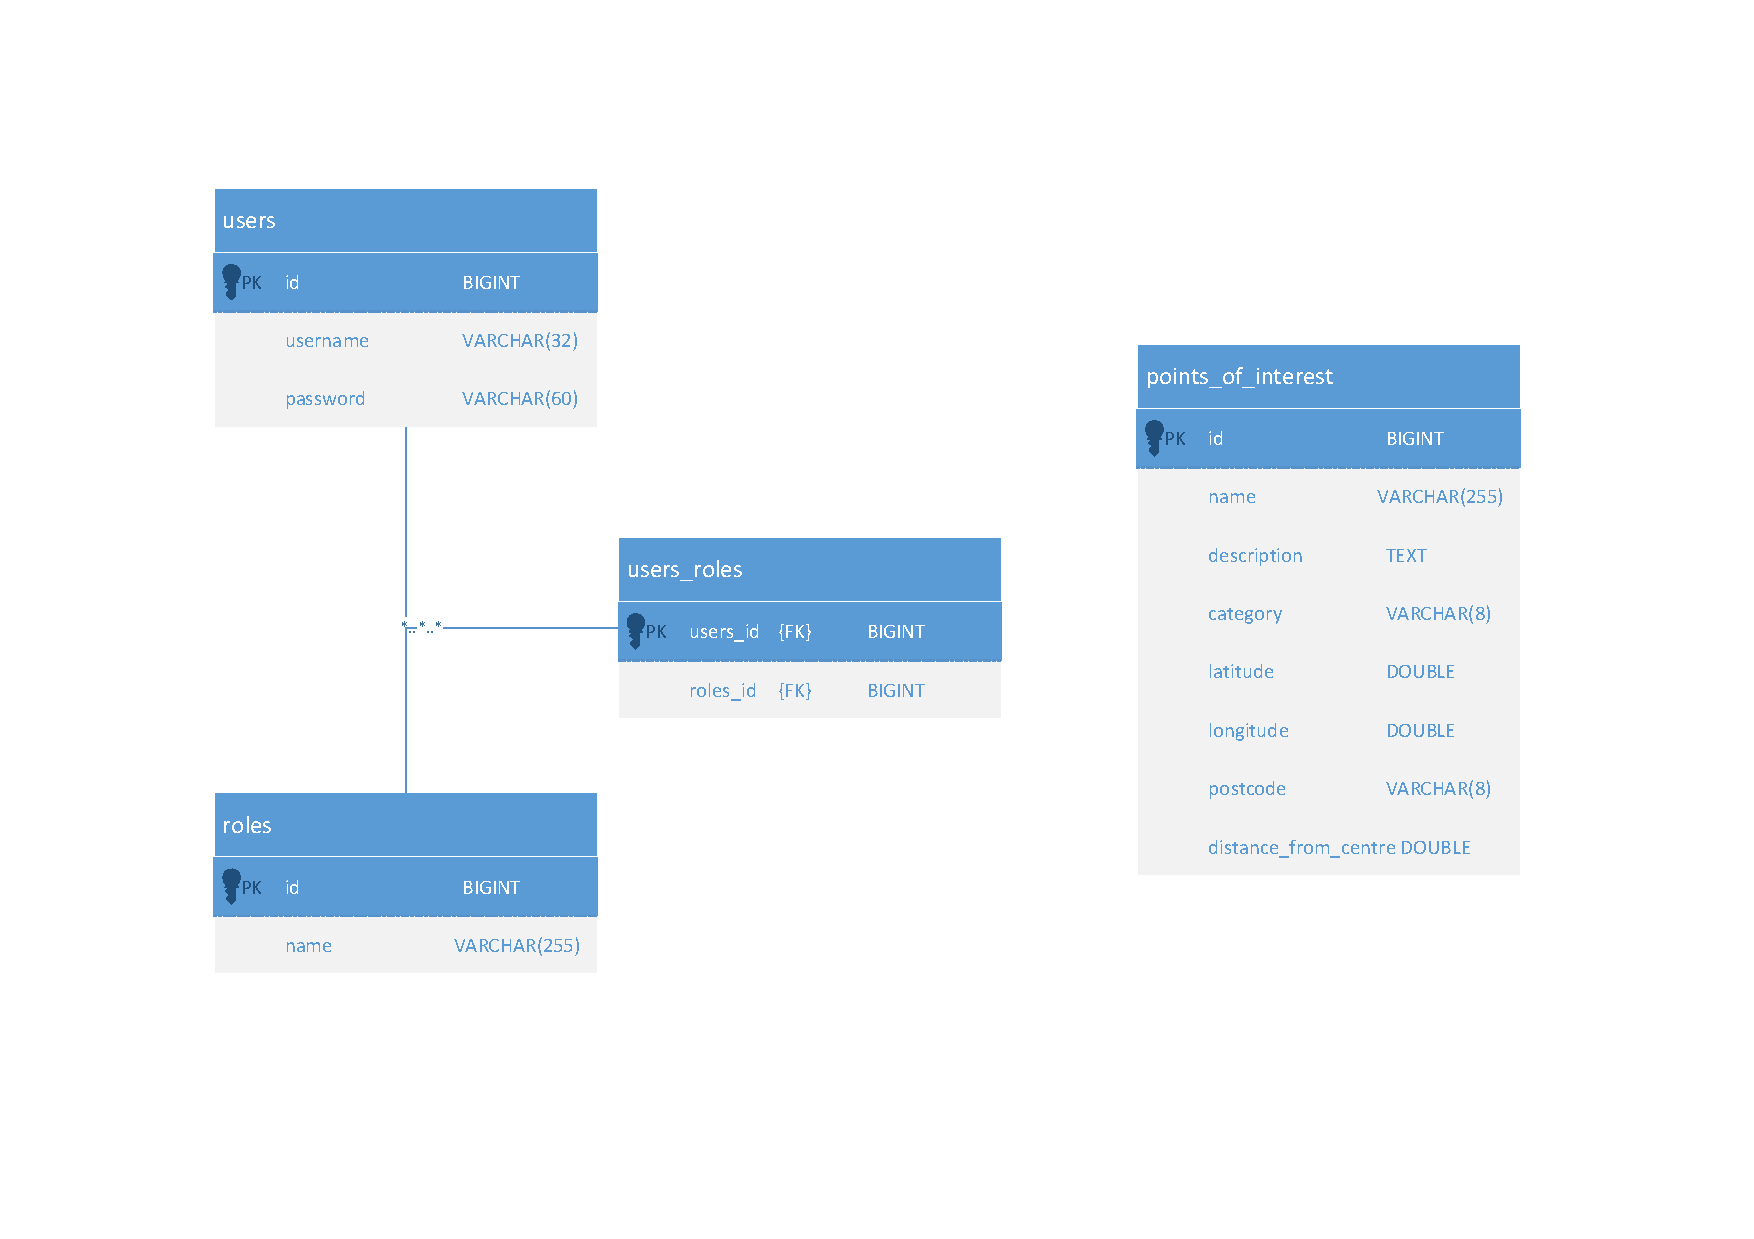
\includegraphics[scale=0.5]{diagrams/er_diagram}
\end{figure}	

Ultimately, the database design was uncomplicated, as there were only three objects to consider. As the majority of database handling was intended to be carried out through the Spring Data JPA, the nuances that that brings were added into the database at time of design. One example would be the ID primary key on each relation. In a standard PostgreSQL database implementation, the data type of the ID is not likely to be of type \textit{bigint}. This is a type that is, as the name implies, intended for large integers. An ID attribute that is being utilised as a primary key would generally take the type of \textit{serial} - an auto-incrementing column. This is, however, handled within the backend by the JPA, through an automatically-generated sequence stored within the database, therefore there is no need to use the serial type.

A many-to-many relationship between both users and roles is achieved through the use of a junction able, \textit{users\_roles}. This allows for multiple roles to be added into the database at a later date, which can then be attributed to users through the frontend. As each user is only permitted to have one role, the primary key has been set as the user in the junction table, with a role ID being set with each user.

\subsection{Constraints}

Constraints had to be created in order to validate the data that was being entered into the table, this is described below, with the definition in a pseudo-code format:

% Please add the following required packages to your document preamble:
% \usepackage{graphicx}
\begin{table}[h]
\centering
\resizebox{\textwidth}{!}{%
\begin{tabular}{|l|l|}
\hline
\textbf{Constraint Name}                   & \textbf{Definition}                                    \\ \hline
\textbf{latitude\_chk}                     & CHECK latitude IS \textgreater -90 AND \textless 90    \\ \hline
\textbf{longitude\_chk}                    & CHECK longitude IS \textgreater -180 AND \textless 180 \\ \hline
\textbf{latitude\_not\_null\_island\_chk}  & CHECK latitude NOT EQUAL TO 0                        \\ \hline
\textbf{longitude\_not\_null\_island\_chk} & CHECK longitude NOT EQUAL TO 0                        \\ \hline
\textbf{chk\_name}                         & CHECK name IS NOT EMPTY                                \\ \hline
\textbf{postcode\_chk}                     & CHECK postcode MATCHES UK postcode regex               \\ \hline
\end{tabular}%
}
\caption{A list of constraints in the points\_of\_interest relation}
\label{poi_constraints}
\end{table}

These constraints tend to perform sanity checks on the input that is being entered, once it reaches the database layer. The constraints on the coordinates are based upon the natural constraints based upon latitude and longitude, and ensures that a user cannot apply an incorrect coordinate to a point of interest, that would likely cause an error at the frontend layer of the application.

The two ``not null island" checks make sure that a user cannot simply enter 0 as the latitude and 0 as the longitude, as this could potentially cause issues when parsing the postcode in the backend layer. The primary issue with a check like this would be that 0,0 is a valid coordinate pair. However, the customer has specified that points of interest would primarily be in the United Kingdom, which is far from this coordinate range. It is not likely that any potential coordinate pairs entered for points of interest outside the UK would be equal to these coordinates.

A regular expression, sought from an open data source that provides APIs dealing with UK postcodes\cite{PostcodeRegex}, was, again, a sanity check. It performs basic error-checking that checks the general shape of the postcode; checking it has a letter at the beginning and ends in a letter, for example. Whilst stricter regular expressions were available, these were often rather complex expressions that were computationally intensive, and still did not cover every edge case, often making their implementation futile. The design accounts for error-checking of postcodes through the use of the aforementioned API, which is further explained in section~\ref{sec:backend}. 


\section{Backend}
\label{sec:backend}

\begin{figure}[!ht]
	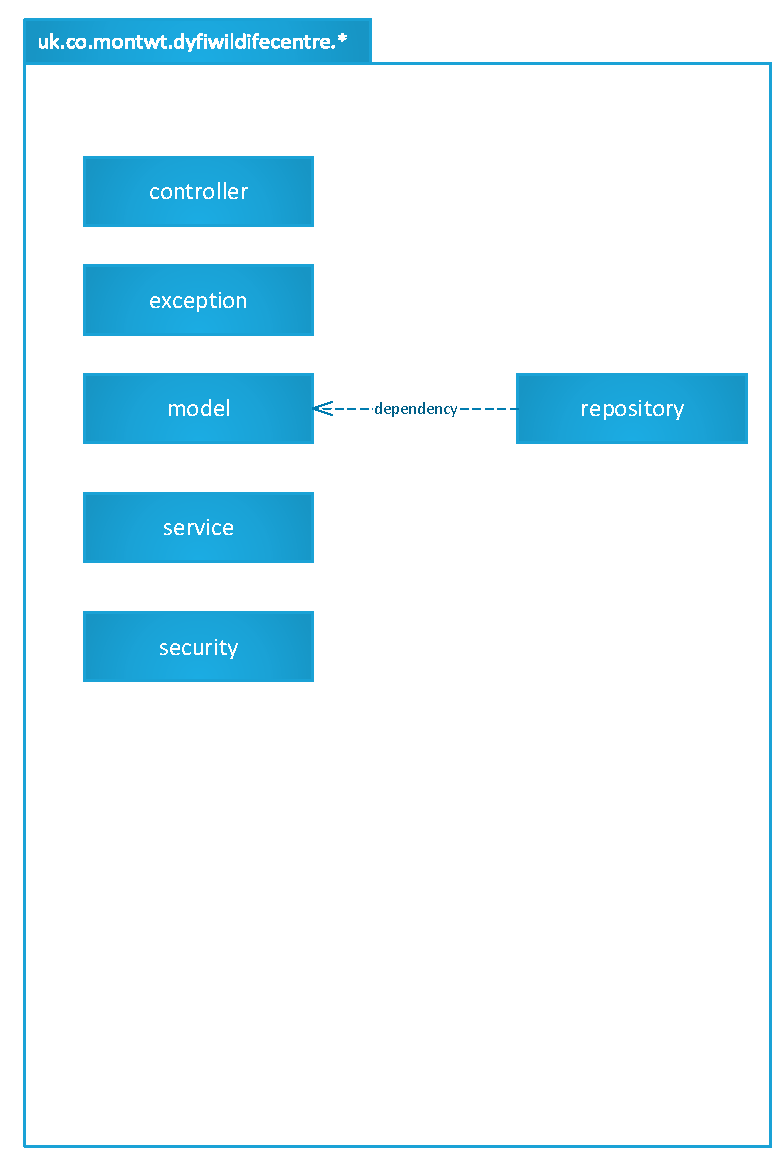
\includegraphics[scale=0.5]{diagrams/parent_uml}
	\caption{Parent UML diagram, showing each package that the software breaks down into}
\end{figure}	

Spring, the framework that is utilised in this backend, follows a model-view-controller design pattern. This allows for a clear distinction between each area of the application, with its functionalities and design being defined as follows:

\begin{itemize}
	\item	\textbf{Model} - The application's data structure and logic processing, containing the objects representing a user, a role, and a point of interest. It also includes a repository layer, that interfaces with the PostgreSQL server, and a service layer, that provides a layer of abstraction between the database and the controller.
	\item	\textbf{View} - The presentation of data in the application. This is generally further discussed in Section~\ref{sec:frontend}, but there are a number of classes and configurations that directly affect the management of the view layer.
	\item	\textbf{Controller} - Classes that accept user and computer input, converting it to commands that affect either the model or the view. In this application, the controller consists of a RESTful API for managing users and points of interest.
\end{itemize}

Class diagrams were created to be adhered to during the production of this application, and were split by layer. The intention was for Java packages to be used, to aid in code navigability and ease of maintenance. %1245 words

\subsection{Model layer}


\subsection{View Layer}


\subsection{Controller Layer}


\subsection{Security}

\section{Frontend}
\label{sec:frontend}

\subsection{Design considerations}

\subsection{Prototyping}

\subsubsection{Home Screen}
% Figure of home screen

% Figure of home screen with hamburger menu

\subsubsection{Marker information}
% POI card

\subsubsection{Admin Panel - Login Screen}
% Admin Login
\subsubsection{Admin Panel - POI editing}

\subsubsection{Admin Panel - User management}
